\chapter{Passiv Radar Setup}
\section{Einführung}
\section{Hardware}
\subsection{ADALM-Pluto SDR}
Bei dem hier verwendeten SDR handelt es sich um ein ADALM
PLUTO SDR. Der Hauptgrund, warum sich in diesem Versuchsaufbau für dieses Gerät entschieden wurde ist die Bandbreite dieses Gerätes die bei bis zu 20 MHz liegt. Die Bandbreite des Signals was hier für Passiv Radar verwendet beträgt nämlich 5MHz was einige SDR nicht aufbringen können.  Aufs weitere besitzt das SDR eine Frequenz Abdeckung von 325 MHz bis zu 3.8 MHz. Die weiteren Daten können in der Tabelle abgelesen werden.

\subsubsection{Synchronität}
Zur Aufnahme des Referenzsignals als auch des reflektierten Signals werden jeweils ein Pluto-SDR benötigt, diese zwei müssen nun synchron betrieben werden. Dies wird erreicht durch Daisy Chaining  der beiden Uhren der SDRs und einer externen Uhr. Abbildung zeigt dann den fertigen Aufbau der Beiden SDRs und im Schaltplan in Abbildung ist zur erkennen wie die Uhr der jeweiligen SDRs aufgebaut ist.
\subsection{Antenne}
In diesem Aufbau werden zwei Antennen die für DVB-T gedacht sind verwendet. Die Antenne ist ein Yagi Antenne mit 43 Elementen wie man im Abbildung /ref{antenne} sieht die im Frequenzbereich von 470 bis 862 MHZ arbeitet, was für unseren Anwendungsfall sehr gut geeignet ist.Die weiteren Daten zur Antenne stehen in der Tabelle /ref{table:antenne}.

\begin{table}
    \centering
        \begin{tabular}[h]{rl}
            Antenne         & SKT SL43-01 UHF 43            \\
            Antennengewinn  & 11..13 dB                     \\
            Frequenzbereich & 470-862 MHz                   \\
            Halbwertsbreite & horiz. 30...40°/ver. 35...50° \\
        \end{tabular}
    \caption{Daten der SKT SL43-01 UHF 43 Antenne}\label{table:antenne}
\end{table}

\begin{figure}
    \centering
    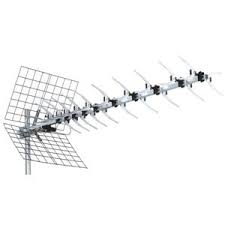
\includegraphics[width=\textwidth]{images/antenne.png}
    \caption{SKT SL43-01 UHF 43 Antenne}\label{antenne}
\end{figure}
\section{Signal}
\subsection{Aufbau von LTE}
\subsubsection{PSS}
\subsubsection{SSS}
\section{Software}

Nachfolgend soll nun die verwendete Softwaresuite erläutert werden. Dazu wird zunächst die zur Aufnahme genutzte Lösung beschrieben. Anschließend wird näher auf die eigens entwickelte Signalverarbeitungskette eingegangen.

\subsection{Aufnahme}

Um Daten vom PlutoSDR zu empfangen bedarf es einer Bediensoftware um den Empfangsprozess zu steuern. Zahlreiche solcher SDR-Anwendungen existieren auf dem Markt, viele davon Open-Source oder als Freeware erhältlich. Der Hersteller selbst, Analog Devices, bietet ein low-level Treiberpaket names \emph{libiio} (der Name setzt sich zusammen aus dem Unix typischen lib-Präfix für \emph{library} und dem Akronym iio---%
% cspell:disable-next-line
\textbf{i}ndustrial \textbf{i}nput/\textbf{o}utput---%
steht) an. Mit diesem ist es möglich lokal-, über USB- oder Netzwerk verbundene ADCs und FPGAs von Analog Devices zu steuern. Das Treiberpaket beinhaltet dabei einige Kommandozeilenanwendungen mit denen angeschlossene Geräte enumeriert, einzelne Register gelesen und beschrieben und die Firmware ak­tu­a­li­sie­rt werden können. Darüberhinaus kann über eine API, die Teil der namensgebenden libiio Bibliothekdatei ist, auf Geräte zugegriffen werden.

Es ist diese API an der die meisten SDR-Anwendungen ansetzten. Welche Funktionen der Hardware dann genau nutzbar sind, hängt von der jeweiligen Anwendung ab. Für die Durchführung dieses Projekts würde sich dabei für die Anwendung SDRangel\footnote{Homepage: \url{https://bit.ly/sdrangel}} von Edouard Griffiths entschieden. Abbildung~\ref{fig:sdrangel_screenshot} zeigt die graphische Oberfläche der Anwendung. Die Software unterstützt das Darstellen und Aufzeichnen von IQ-Rohdaten in einem eigenen Dateiformat. Die Möglichkeit der Live-Darstellung der Daten in Frequenz- und Wasserfalldiagramm hat sich in den Messkampangen als äußerst hilfreich erwiesen.

\begin{figure}[htb]
    \centering
    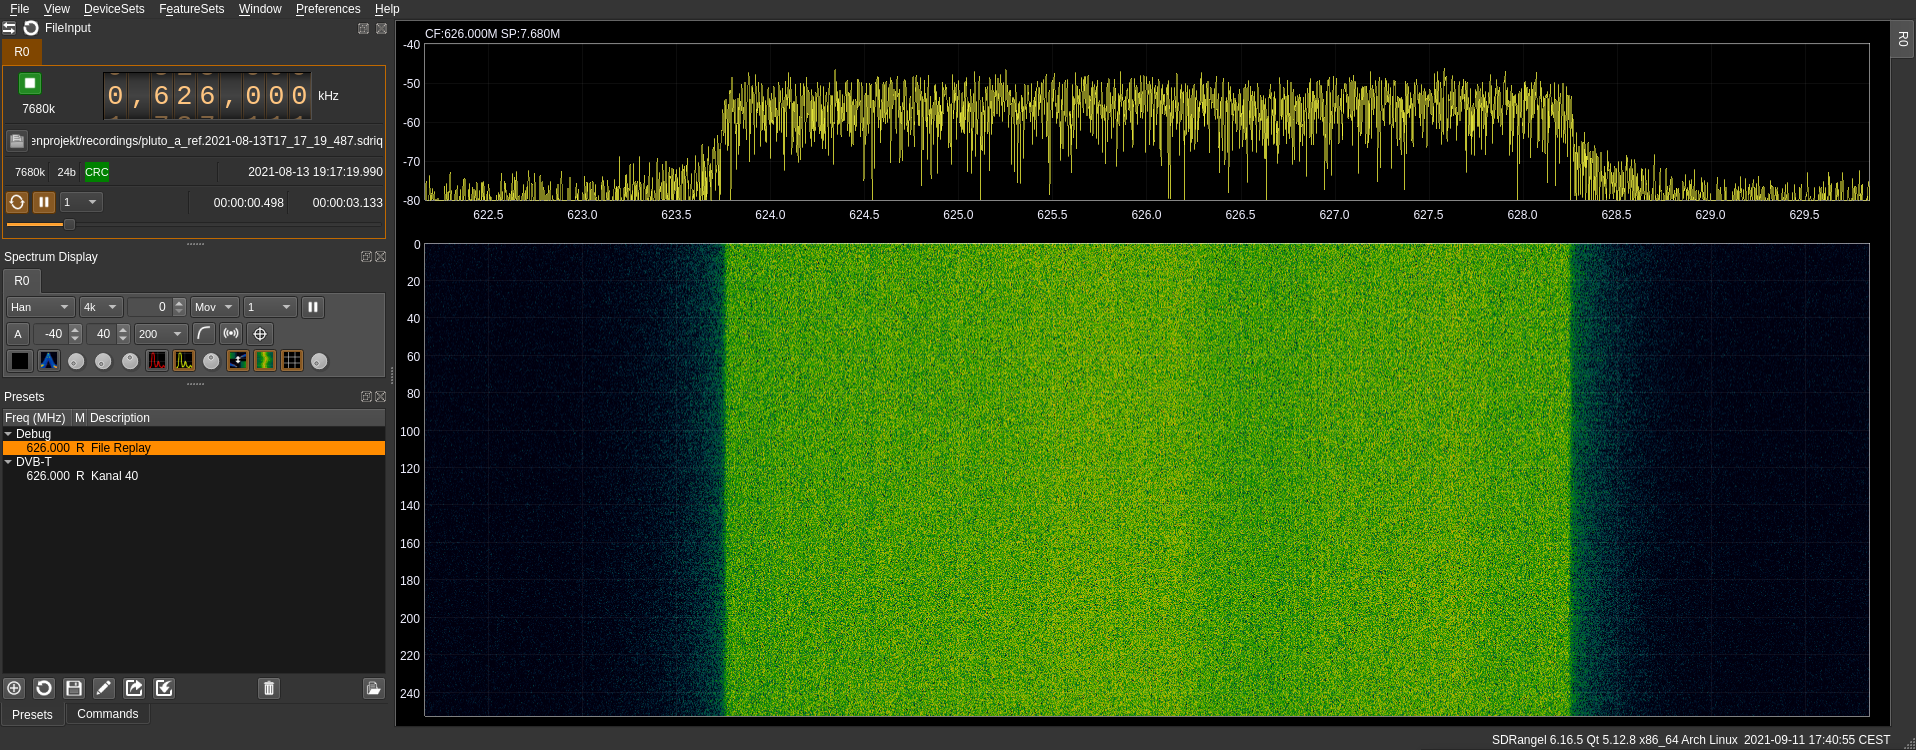
\includegraphics[width=\textwidth]{images/sdrangel.png}
    \caption{SDRangel im Replay-Modus einer zuvor angefertigten Messung.}\label{fig:sdrangel_screenshot}
\end{figure}

Da es sich hierbei um Open-Source-Software handelt, konnten benötigte Funktionen oder Bugfixes\footnote{Liste aller Änderungen: \url{https://bit.ly/sdrangel-pr}} direkt selbst implementiert werden und sind anschließend ins Projekt zurück geflossen. So wurde ein Bugfix zur parallelen Nutzung zweier PlutoSDR erstellt, eingereicht und in den Hauptentwicklungszweig des Ursprungsprojekts aufgenommen.

\subsection{Signalverarbeitung}
\subsubsection{Ambiguity Funktion}\label{sct:ambiguity_function}
\subsubsection{Clean Algorithmus}
